\chapter{Introduction and theory}
\label{chap:theory}

\section{The Standard Model of particle physics}
\subsection{Introduction}

The \SM of particle physics was formulated in the second half of the 20$^{\text{th}}$ century. It has been an immensely successful theory, accurately describing all known processes in high energy physics encountered thus far. The \SM is a gauge theory, in particular a \QFT, in which the universe is made up of interacting fields. In this model, the fundamental elements of matter can be represented as relativistic quantum fields, the excitations of which are manifested as particles. Furthermore, the fundamental forces which govern the interactions of matter can be described the exchange of mediator particles. The \SM places the electromagnetic, strong and weak forces into one framework. The only force which is not described not the \SM is gravity, since no viable quantum theory of gravity currently exists. This does not affect the predictive power of the \SM however, since the gravitational force is many orders of magnitude weaker than the other three. The \SM unites the electromagnetic and weak forces into the electroweak force, using the Higgs mechanism to explain the manifest breaking of the underlying symmetry. The Higgs mechanism leads to the prediction of an observable particle, the Higgs boson. All the particles postulated by the \SM have been discovered, capped by the discovery of the Higgs boson in 2012.

%In order to do this, a mechanism ss required to permit the $W^{\pm}$ and $Z$ vector bosons to have mass while allowing the photon to remain masslesss. Such a theory was independently proposed by several theorists~\cite{BroutEnglert,Higgs1,Higgs2,Kibble1,Higgs3,Kibble2}, and is commonly referred to as the Higgs mechanism. In 1964, Higgs postulated that one outcome of this mechanism was that it should yield an observable particle, the Higgs boson~\cite{Higgs2}.

Although the \SM has been very successful as a theory, it falls short of being a “theory of everything", and is clearly incomplete. For instance, it does not accommodate mass terms for neutrinos, which are required to explain the origin of neutrino oscillations observed in many experiments~\cite{SuperK,SNO,DayaBay}. Furthermore, it does not contain a viable candidate for dark matter, which may be needed to explain the mass deficit of the universe~\cite{DM}. Other issues such as the hierarchy problem~\cite{Hierarchy} and the origin of matter-antimatter asymmetry~\cite{Asymmetry} also persist. Clearly, the \SM is incomplete or approximate, and many efforts in modern high energy physics are being made to discover \BSM physics. Many extensions to the  detailed studies of the properties of the Higgs boson could provide valuable insight into the nature or indeed existence of \BSM physics.

%Over the decades, the particles which constitute the SM were discovered: the $\tau$ lepton in 1975~\cite{tauDisc}, the $b$ quark in 1977~\cite{bquarkDisc}, the gluon in 1979~\cite{Gluon1,Gluon2,Gluon3}, the $Z$ and $W^{\pm}$ bosons in 1983~\cite{ZDisc,WDisc}, the $t$ quark in 1995~\cite{tquarkDisc1,tquarkDisc2} and the $\nu_{\tau}$ in 2000~\cite{TauNuDisc}. By the turn of the millennium, all but one particle postulated by the SM had been observed: the Higgs boson, which had proved elusive despite decades of searches. The Higgs search prompted the construction of the Large Hadron Collider (LHC) at CERN, and two multi-purpose detectors, ATLAS and CMS, were designed with the Higgs observation as one of their main physics goals. In 2012, the two experiments jointly announced the observation of a Higgs-like particle of mass $\sim$125 GeV, ending a 50-year interval between postulation and discovery~\cite{CMSHDisc,ATLASHDisc}.


\subsection{Particles and Forces}

 In the \SM, matter is made up a collection of \SpinHalf particles, which are called \emph{fermions}. Fermions come in two types: those wich interact exclusively via the eletroweak force, known as the \emph{leptons} and those which can also interact via the strong nuclear force, known as the \emph{quarks}. The fermions can be arranged into three \emph{generations}, which are identical copies of each other, aside from the masses of the constituent particles. The first generation includes the electron (\Pe), the electron neutrino (\Pnue), the up quark (\Pup) and the down quark (\Pdown). The second generation includes the muon (\Pmu), the muon neutrino (\Pnum), the charm quark (\Pcharm) and the strange quark (\Pstrange). The third and final generation includes the tau (\Ptau), the tau neutrino (\Pnut), the truth or top quark (\Ptop) and the beauty or bottom quark (\Pbottom). Each of the particles mentioned in the list above has a corresponding \emph{antiparticle}, with the same mass and opposite quantum numbers.
The \SM fermions and their properties are displayed in \Tab~\ref{tab:th:fermions}.

\begin{table}[h!]
 \resizebox{\textwidth}{!}{

\begin{tabular}{ |c | c l | c l | c l | }
\hline
type & \multicolumn{2}{|c}{ Generation I} & \multicolumn{2}{|c}{ Generation II} & \multicolumn{2}{|c|}{ Generation III} \\
\hline
  \multirow{4}{*}{leptons} & \multirow{2}{*}{\Large{\Pe}} & $m=0.511\MeV$ & \multirow{2}{*}{\Large{\Pmu}}  &   $m=105\MeV$ &   \multirow{2}{*}{ \Large{\Ptau}}  &   $m=1777\MeV$  \\
                           &                      &   $q=-1$      &   & $q=-1$    &    & $q=-1$   \\ \cline{2-7}
                           & \multirow{2}{*}{\Large{\Pnue}} & $m\sim0\MeV$ & \multirow{2}{*}{\Large{\Pnum}}  &   $m\sim0\MeV$ &   \multirow{2}{*}{ \Large{\Pnut}}  &   $m\sim0\MeV$  \\
                           &                      &   $q=0$      &   & $q=0$    &    & $q=0$   \\
 \hline 
  
  \multirow{4}{*}{quarks} & \multirow{2}{*}{\Large{\Pup}} & $m=2.3\MeV$ & \multirow{2}{*}{\Large{\Pcharm}}  &   $m=1.275\GeV$ &   \multirow{2}{*}{ \Large{\Ptop}}  &   $m=173\GeV$  \\
                           &                      &   $q=+\frac{2}{3}$      &   & $q=+\frac{2}{3}$    &    & $q=+\frac{2}{3}$   \\ \cline{2-7}
                           & \multirow{2}{*}{\Large{\Pdown}} & $m=4.8\MeV$ & \multirow{2}{*}{\Large{\Pstrange}}  &   $m=95\MeV$ &   \multirow{2}{*}{ \Large{\Pbottom}}  &   $m=4.18\GeV$  \\
                           &                      &   $q=-\frac{1}{3}$      &   & $q=-\frac{1}{3}$    &    & $q=-\frac{1}{3}$   \\
 \hline 
  \end{tabular}
}
 \caption{The fundamental \SM particles which constitute all matter in the universe are presented. There are three generations of matter, which are identical copies of each other aside from the mass of the constituent particles. Each generation has two leptons and two quarks. The mass $m$ and electric charge $q$ are indicated for each particle. For every particle in the table, there exists an antiparticle with the same mass but opposite quantum numbers. }
\label{tab:th:fermions}
\end{table}

The fundamental matter particles described above interact via the fundamental forces. There are four known fundamental forces in the universe: the electromagnetic force, the weak nuclear force, the strong nuclear force and the gravitational force. The gravitational force is many orders of magnitude weaker than any of the other forces, and therefore has a negligible effect on the interactions of the \SM particles. Furthermore, no adequate quantum theory of gravity currently exists, therefore it cannot be easily included in the \SM. Therefore, the \SM deals only with the strong, weak and electromagnetic forces.

In the \SM, the fundamental forces, are represented by the exchange of\emph{mediator particles}. In contrast to the \emph{fermions}, the mediators have integer spin. Integer-spin particles are referred to as \emph{bosons}, and in particular the force carriers have spin 1, making them \emph{vector bosons}. 
Each fundamental force is mediated by one or more vector bosons. The electromagnetic force is mediated by the photon (\Pphoton). The weak nuclear force is mediated by the Z-boson (\PZ) and the W-bosons (\PWplus and \PWminus). The strong nuclear force is mediated by the gluons (\Pgluon), of which there are eight, one for each possible colour charge (the strong force equivalent of electric charge).
The forces described by the \SM, along with their mediators, are shown in \Tab~\ref{tab:th:bosons}.

\begin{table}[h!]
 \resizebox{\textwidth}{!}{
\begin{tabular}{ |c | c  | c  | c|  }
\hline
Force &  Indicative Strength & Mediator & Mass  \\
\hline
strong &  $1$ & gluon \Pgluon & 0   \\
\hline
electromagnetic &  $10^{-3}$ & photon \Pphoton & 0   \\
\hline
 \multirow{2}{*}{weak} &  \multirow{2}{*}{$10^{-8}$} & W-boson \PWpm & 80.4 \GeV   \\
                       &                             & Z-boson \PZzero & 91.2 \GeV   \\
\hline
  \end{tabular}
}
 \caption{The three fundamental forces considered by the \SM are presented. For each force, the approximate strength relative to the strong force is shown, assuming two fundamental particles separated by a distance of $10^{-15}\m$. The mediator particle of each force is indicated along with its measured mass.\cite{Thomson:2013zua}}
\label{tab:th:bosons}
  \end{table}

The \Pphoton and \Pgluon are massless, in contrast to the \PWmp and \PZzero, which are massive. This difference is explained via the process of \emph{electroweak symmetry breaking} via the Brout-Englert-Higgs mechanism described in \Sec~\ref{src:th:ewsb}. This mechanism introduces an additional field, which leads to an additional massive observable particle, the Higgs boson. This particle is predicted to be spin-$0$, and therefore it is referred to as a \emph{scalar boson}.

\subsection{Gauge groups of the SM Lagrangian}
\label{sec:th:gauge}

Typically, QFTs are expressed in the Lagrangian formalism. The Lagrangian $\mathcal{L}_{\text{QFT}}$ of a \QFT codifies the dynamics and interactions of its particles. The equations of motion can be extracted using the \ELE. $\mathcal{L}_{\text{QFT}}$ is constructed by considering the nature of the particles involved in the \QFT and imposing the symmetries which the theory ought to display. N\"other's Theorem~\cite{Noether}, one the most important in the study of particle physics, shows a profoudn relationship between the symmetries of a problem and the laws which govern it: for every symmetry in a Lagrangian, there is an associated conservation law. For example, if we impose that our \QFT should be invariant in time or space, this directly implies that the theory respects conservation of energy or momentum respectively. Similarly, if the \QFT is invariant under rotations in space, angular momentum is conserved. These simple examples illustrate that imposing a symmetry in a Lagrangian will place requirements on how the particles in the theory are allowed to propagate and interact. 

A gauge theory is a particular type of \QFT where local gauge transformations are a symmetry of the Lagrangian. Such gauge symmetries are of principal importance in particle physics, as they lead to the introduction of gauge fields, and thus the gauge bosons which are the mediators of a force. The \SM is in fact a collection of gauge theories. In this case a gauge transformation takes the form of shifting the quantum mechanical phase of all wavefunctions. It is reasonable to require such transformations to leave the dynamics of the theory intact, since the phase of a wavefunction is never manifest in a physical observable. Thus the Lagrangian of any realistic theory should be \emph{gauge invariant}, i.e. symmetric under gauge transformation operations.  

A simple example is \QED, where for simplicity we consider a single fermion (others can be trivially added). Fermions are described by the Dirac equation, which, in the Lagrangian formalism, takes the form:

\begin{equation}
\label{eq:th:dirac}
\mathcal{L}_{\textrm{fermion}} = i\overline{\psi} \gamma^{\alpha} \partial_{\alpha} \psi - m\overline{\psi}\psi,
\end{equation}

where i is the imaginary unit, $\psi$ is a Dirac spinor and $\overline{\psi}$ is its adjoint, $m$ is the mass of the fermion, $\gamma^{\alpha}$ represents the Dirac gamma matrices and $\partial_{\alpha}$ is the 4-gradient. 
Requiring \emph{global} gauge invariance means that we require that the Lagrangian is invariant under a global phase transformation $\psi \rightarrow \psi'= \psi e^{i\theta}$, where $\theta$ is constant in time and space. This requirement is trivially satisfied by $\mathcal{L}_{\textrm{fermion}}$ :
$$
\mathcal{L}_{\textrm{fermion}} \rightarrow \mathcal{L}_{\textrm{fermion}}'=i\overline{\psi e^{i\theta}} \gamma^{\alpha} \partial_{\alpha} \psi e^{i\theta} - m\overline{\psi e^{i\theta}}\psi e^{i\theta}  =i \overline{\psi } e^{-i\theta} e^{i\theta}\gamma^{\alpha} \partial_{\alpha} \psi - m\overline{\psi} e^{-i\theta} e^{i\theta}\psi  = \mathcal{L}_{\textrm{fermion}},
$$
where it was possible to move $\psi e^{i\theta}$ from the left to teh right of the 4-gradient because $\theta$ is a constant.However, there is no particular reason to apply the same transformation throughout space and time. Indeed, the theory should also be invariant under \emph{local} phase transformations $\psi \rightarrow \psi'= \psi e^{i\theta(\vec{x},t)}$.


\subsection{Electroweak Symmetry Breaking}
\label{sec:th:ewsb}

\section{The Higgs boson}
According to SM, the Higgs boson's coupling with particles is proportional to their masses. As such, its production modes in the environment of the LHC are dominated by interactions involving the heavier particles of the SM. Typically, the Higgs boson is produced by one of the following mechanisms (Fig. \ref{higgs_prod}, whose cross-sections can be seen in Fig. \ref{H_XS_fig}):

  \begin{figure}[h!]

  \centering
  \subfloat[]{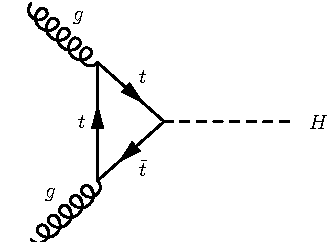
\includegraphics[width=0.3\textwidth]{theoryFigures/ggH.pdf}}
  \subfloat[]{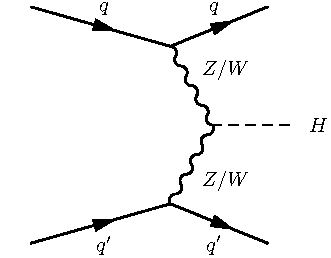
\includegraphics[width=0.3\textwidth]{theoryFigures/vbf.pdf}}\\
  \subfloat[]{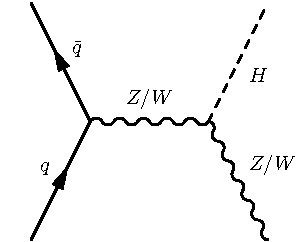
\includegraphics[width=0.3\textwidth]{theoryFigures/wzH.pdf}}
  \subfloat[]{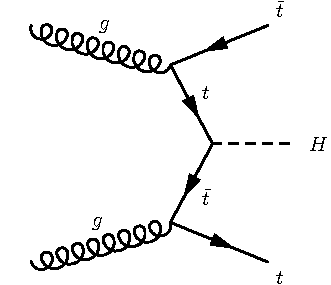
\includegraphics[width=0.3\textwidth]{theoryFigures/ttH.pdf}}
  \caption{Higgs production modes at the LHC: (a) gluon-gluon fusion, via a loop of top quarks, (b) vector boson fusion (VBF), with associated quark production, (c) associated vector boson production and (d) top quark fusion with associated top quark production. }
  \label{fig:theory:higgsproduction}
  \end{figure}

  \newpage
  By the same token, the SM Higgs boson decays to pairs of particles with branching ratios proportional to the square of their mass. The production of a pair of $t$ quarks is not kinematically allowed because their mass is high, so the most likely decay modes are $H \rightarrow ZZ \text{, } W^{\pm}W^{\mp}$, $ b\bar{b}$ and $ \tau^+ \tau^-$. In addition, a small fraction of decays of the Higgs boson ($<1\%$, see Fig. \ref{H_BR_fig}) can occur via a loop diagram to a pair of high-energy photons. The branching fractions and cross sections of these production and decay modes are available in the Handbook of LHC Higgs Cross Sections~\cite{H_XS1,H_XS2}.


  The Higgs boson was discovered in 2012 using data from runs at $\sqrt{s}=7$ and $8$ TeV, and was found to have a mass $m_H \sim 125$ GeV. The signal strengths of the various decay modes at the CMS and ATLAS experiments can be seen in Fig. \ref{sig_strength}. Despite fewer than $1\%$ of Higgs boson decays occurring via $H \rightarrow \gamma \gamma$, this channel played a crucial role in the discovery, and remains one of the two most sensitive methods of studying the Higgs boson. This is in part thanks to the excellent performance of the CMS and ATLAS ECALs, which were able to reach similar sensitivities to the $H\rightarrow \gamma \gamma$ decay mode.

  \subsection{History of Higgs boson searches}
  \subsection{Higgs boson at the LHC}
